\section{Introdução e Justificativas}\label{Intro}


%=============================================================================
% 							INTRODUÇÃO
%=============================================================================

%GFC E QUESTIONAMENTO DO INVESTIMENTO COMO CAUSA CAUSANS
PALAVRA INICIAL 
Os impactos sócio-econômicos da Crise Financeira Global (CFG) são imensuráveis, mas algumas das mudanças sobre a teoria econômica já podem ser tateadas. Se, por um lado, abalou a macroeconomia ortodoxa ao ponto da política fiscal estar sendo repensada, por outro, redirecionou algumas pautas na heterodoxia. Distribuição e desigualdade, temas tão caros a esta última tradição, ganharam novo fôlego enquanto parte da literatura passou a destacar o consumo como um dos possíveis motores de crescimento (MACEDO e LIDIA). Desse modo, umas das consequências da CGF é a reavaliação do investimento das firmas enquanto  ``a causa das causas''. Paralelamente, verificou-se um crescente interesse nas implicações macroeconômicas do investimento residencial\footnote{E isso é verificado até na literatura ortodoxa. Inspecionando modelos DSGE que incluem investimento residencial, \textcite{iacoviello_housing_2010} conclui que um melhor entendimento dos impactos deste gasto se faz necessária para a compreensão das flutuações macroeconômicas. } (FIEBIGER). 

Neste ponto, cabe mencionar o ineditismo de \textcite{green_follow_1997} e \textcite{leamer_housing_2007} --- e revisitado em \textcite{leamer_housing_2015} e por \textcite{fiebiger_trend_2017} --- ao lançar luz sobre a importância do investimento residencial na determinação dos ciclos econômicos antes da crise dos \textit{subprimes}. Ao avaliar o caso norte-americano, \textcite{green_follow_1997} conclui que o investimento residencial possui uma capacidade preditiva maior que o investimento das firmas, mas que isso não implica no estabelecimento de uma relação causal. Na tentativa de compreender tais resultados, afirma:

\begin{quote}
	
	[P]erhaps residential investiment, like stock prices and interest rates, is a good predictor of GDP because it is a series that reflects \textbf{foward looking behavior}. Presumably households will not increase their expenditures on housing unless they expect to prosper in the future. Building a house is a natural mechanism for doing this. Thus, the series can do a good job of predicting GDP without necessarily causing GDP.
	\cite[p.~267, grifos adicionados]{green_follow_1997}
\end{quote}
\textcite{leamer_housing_2007}, por sua vez, avança em direção a relação de causalidade entre este gasto e o PIB. Grosso modo, afirma que a construção de novos imóveis implica em maior consumo de bens duráveis e, portanto, trata-se de um ciclo decorrente do \textit{volume} e não do preço dos imóveis. MAIS REFERÊNCIAS SOBRE EUA.

Além disso, parte da literatura empírica recente também têm lançado luz sobre a importância deste gasto para o ciclo econômico. \textcite{alvarez_does_2010}, por exemplo, concluem que tal tipo de investimento antecede o ciclo econômico para o caso de espanhol e resultados semelhantes podem ser encontrados para França \cite{ferrara_cyclical_2010}, Espanha  e Itália enquanto o caso alemão apresenta uma dinâmica distinta \cite{ferrara_common_2010}. 
Outros estudos, por sua vez, têm enfatizado o efeito riqueza sobre o consumo e indicam tais canais de transmissão são mais incidentes, em ordem, sobre Estados Unidos e Grã Bretanha mas mais brandos no caso francês e alemão \cites{sastre_assessment_2010}{chauvin_wealth_2010}{bassanetti_effects_2010}{arrondel_housing_2010}. Por fim, \textcite{huang_is_2018} testam ambas as hipóteses aventadas por Leamer  (predição e causalidade) e concluem que: (i) o investimento residencial não é um mero canal de transmissão da política monetária; (ii) a construção de novos imóveis tem maior capacidade preditiva que os preços; (iii) o preço dos imóveis tem maior influência no longo prazo e (iv) os resultados sobre a relação de causalidade não são conclusivos para todos os países dada heterogeneidade institucional.

A pluralidade de resultados reportada acima sugere que a especificidade institucional de cada país desempenha um papel central nas implicações macroeconômicas do investimento residencial e, portanto, carece de uma análise mais pormenorizada. A título de exemplo, o caso alemão se destoa dos demais por ALEMANHA. 

INVESTIMENTO RESIDENCIAL, INSTITUCIONALIDADE: Van guten

\begin{table}[htb]
	\centering
	\caption{Características institucionais de alguns países europeus}
	\label{Institucional}
	\resizebox{\textwidth}{!}{%
		\begin{tabular}{l|c|c|c|c|c|c}
			\hline \hline\\
			\textbf{Fatores institucionias}                                                              & \multicolumn{1}{c}{\textbf{França}} & \multicolumn{1}{c}{\textbf{Alemanha}} & \multicolumn{1}{c}{\textbf{Itália}} & \multicolumn{1}{c}{\textbf{Holanda}} & \multicolumn{1}{c}{\textbf{Portugal}} & \multicolumn{1}{c}{\textbf{Espanha}} \\
			\hline\textbf{Microeconômicos}                                                                     &                                     &                                       &                                     &                                      &                                       &                                      \\
			Maturidade da hipoteca                                                                       & 19                                  & 25-30                                 & 22                                  & 30                                   & 30-40                                 & 30                                   \\
			Tipo de taxa de juros                                                                        & Fixa                                & Fixa                                  & Variável                            & Fixa                                 & Variável                              & Variável                             \\
			\begin{tabular}[c]{@{}l@{}}Reembolso antecipado:\\ Contrato (C)/ Legislação (L)\end{tabular} & C/L                                 & C/L                                   & L                                   & C                                    & L                                     & C/L                                  \\
			\begin{tabular}[c]{@{}l@{}}Retirada de capital próprio \\ (Permissão)\end{tabular}           & Não                                 & Não                                   & Não                                 & Sim                                  & -                                     & Limitado                             \\
			\hline\textbf{Macroeconômicos}                                                                     &                                     &                                       &                                     &                                      &                                       &                                      \\
			\begin{tabular}[c]{@{}l@{}}Financiamento pelo \\ mercado de capitais\end{tabular}            & 12\%                                & 14\%                                  & 20\%                                & 25\%                                 & 27\%                                  & 45\%                                 \\
			Taxa de subsídios                                                                            & 0,54                                & 0                                     & 0,15                                & 1,62                                 & 0,23                                  & 0,6                                  \\
			\begin{tabular}[c]{@{}l@{}}Execução hipotecária: \\ duração (meses)\end{tabular}             & 20                                  & 9                                     & 56                                  & 5                                    & 24                                    & 8 \\ \hline\hline                                 
		\end{tabular}%
	}
\end{table}



Pontuada a importância deste gasto, cabe inspecionar a forma com que a heterodoxia tratou do tema. Parte significativa desta literatura  --- emergente no pós-crise imobiliária --- centra esforços na conexão deste tipo de gasto com processos mais gerais como a financeirização \cites{aalbers_financialization_2008}{bibow_financialization_2010} enquanto uma fração minoritária o relaciona com as variabilidades de capitalismo e as relações com o \textit{welfare state}. Uma análise alternativa é da  ``hipotecarização'' desenvolvida por \textcite{jorda_great_2014} que destaca a crescente participação das hipotecas nos balanços patrimoniais dos bancos como pode ser visualizado no gráfico BLABLA. DESENVOLVER MAIS HIPOTECARIZAÇÃO  E FALAR QUE VAI SER INVESTIGADA.


\begin{figure}
	\centering
	\caption{Participação do empréstimo imobiliário no total do balanço patrimonial dos bancos (1880-2016)}
	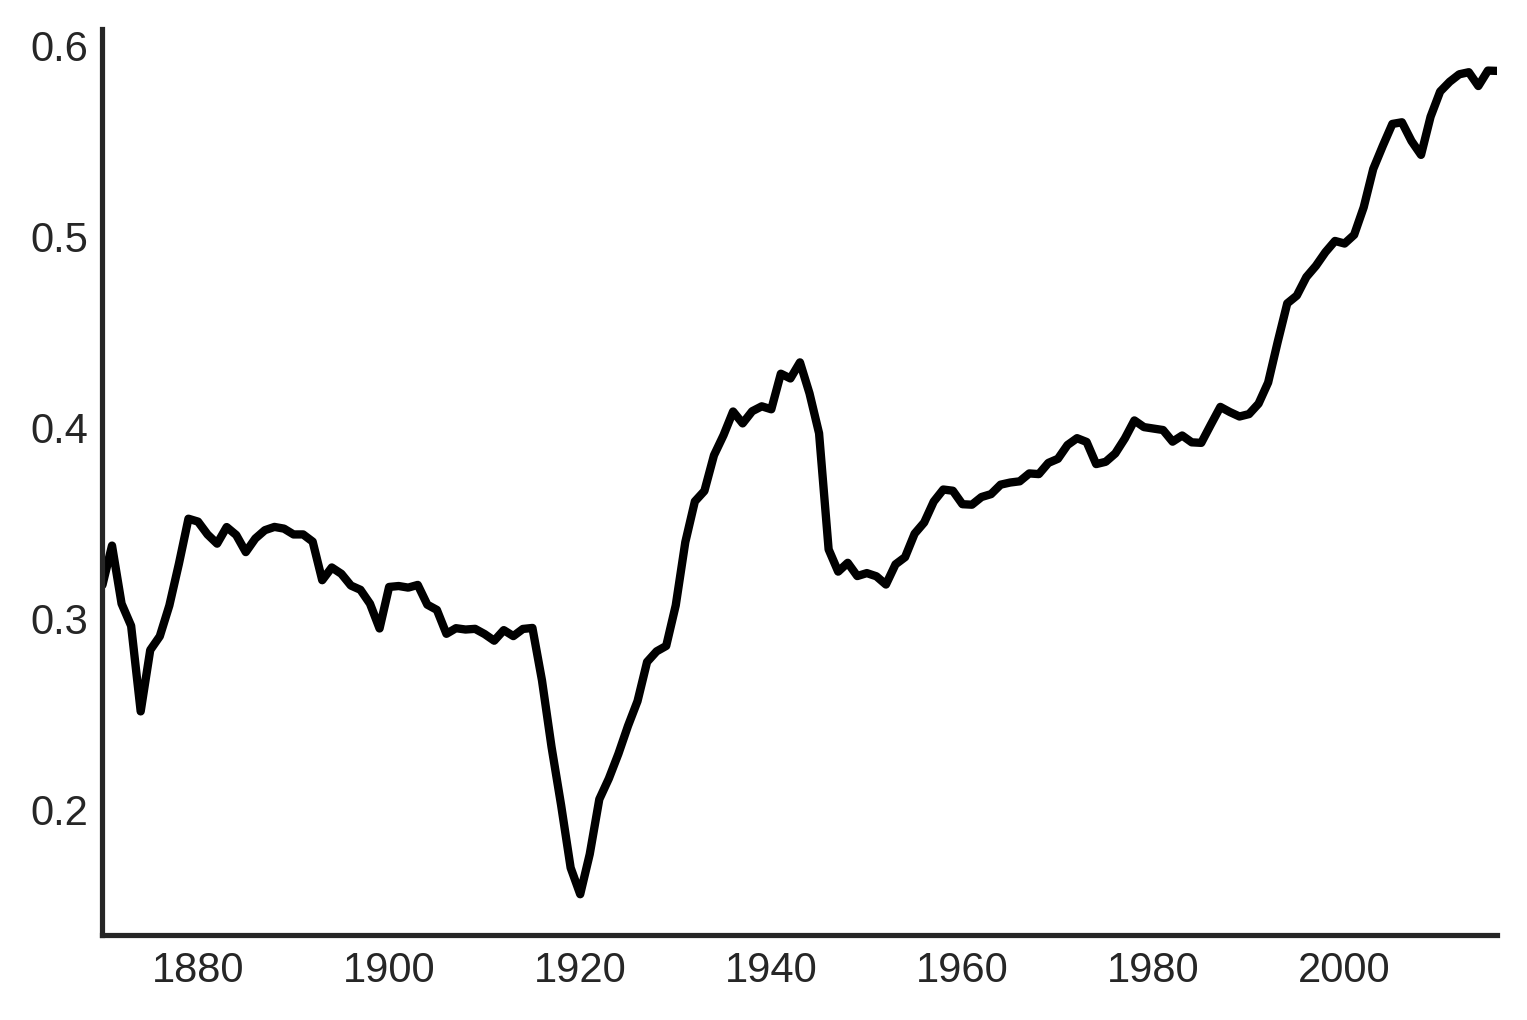
\includegraphics{Jorda_Mean.png}
	\caption*{\textbf{Fonte:}}
\end{figure}

Da revisão bibliográfica, verificou-se que uma fração pequena da literatura heterodoxa\footnote{
	A título de menção, vale destacar também o trabalho de \textcite{zezza_u.s._2008} em que são investigados os efeitos distributivos sobre o crescimento para a economia norte-americana a partir da metodologia \textit{Stock-Flow Consistent}.}
aborda as relações entre crescimento e investimento residencial cujo debate centrado na década de 60-70\footnote{Para mais detalhes, ver \textcite{arku_housing_2006}.} se restringiu em categorizá-lo como um gasto absorvedor de recursos produtivos \cite{solow_importance_1995} e indicava  a possibilidade de um sobreinvestimento residencial \cite{mills_has_1987}. Desse modo, a literatura do supermultiplicador é um contraponto ao \textit{trade-off} apontado por \textcite{solow_importance_1995} uma vez que são os gastos autônomos que lideram o crescimento no longo prazo. Nesta família de modelos, 

FALAR MAIS SUPER

Uma forma de conectar o investimento residencial com o modelo do supermultiplicador sraffiano é por meio da taxa própria de juros dos imóveis (Taxa Própria) desenvolvida por \textcite{teixeira_crescimento_2015} para avaliar o caso norte americano e é definida como a taxa de juros hipotecária ($r_{mo}$) deflacionada pela inflação dos imóveis ({$\dot p_h$}) de modo que o investimento residencial, autônomo e não criador de capacidade produtiva, cresce a taxa $g_Z$ dada por:
\begin{equation}
g_Z = \phi_0 - \phi_1 \overbrace{\left(\frac{1+r_{mo}}{1+\dot p_h} - 1\right)}^{\text{Taxa Própria}}
\end{equation}
em que os $\phi_i$s são parâmetros e cujo termo em parênteses é a Taxa Própria. 


Seguindo a linha argumentativa de \textcite{teixeira_crescimento_2015}, ao evidenciar os impactos da especulação com o estoque de imóveis existente, tal proposta lança luz sobre a influência da inflação imobiliária na construção de novos imóveis e, de acordo com o supermultiplicador sraffiano, sobre o produto como um todo. Em outras palavras, a taxa de juros das hipotecas capta o serviço da dívida para os ``investidores'' (neste caso, famílias) enquanto a variação do preço dos imóveis permite incorporar mudança no patrimonio líquido. Portanto, aufere de modo satisfatório o custo real em imóveis de se comprar imóveis \cite[p.~53]{teixeira_crescimento_2015}. Desse modo, a partir da taxa própria de juros do imóveis é possível revelar importância do investimento residencial para além do ciclo e estendê-la para o longo prazo.  

Como mencionado anteriormente, a referida taxa própria dos imóveis foi desenvolvida para examinar a bolha de ativos ocorria nos EUA e, portanto, requer uma maior investigação a despeito da aplicabilidade para outros países e este é um dos objetivos desta pesquisa (Ver seção BLA). Além disso, uma vez que a dívida hipotecária é o principal componente do endividamento das famílias, se faz necessária uma melhor compreenssão da conexão entre o investimento residencial com as formas de financiamento e estoques financeiros de forma integrada. Nesses termos, a abordagem \textit{Stock-Flow Consistent} se mostra a mais adequada para este tipo de análise (Ver seção Bla).

SFC E SSM COMO ALTERNATIVA

PERGUNTA

Portanto, a presente investigação estende as contribuições de \textcite{serrano_sraffian_1995} ao incluir o investimento residencial na agenda de pesquisa do supermultiplicador sraffiano tal como em \textcite{da_silveira_investimento_2019}, de \textcite{teixeira_crescimento_2015} ao incorporar o conceito de taxa própria de juros dos imóveis para avaliar a dinâmica de tal gasto autônomo, de \textcite{brochier_supermultiplier_2018} por adicionar um tratamento adequado das relações financeiras no SSM por meio da metodologia SFC 
e a de \textcite{jorda_great_2014} ao lançar luz sobre o processo de ``hipotecarização''. 




\begin{comment}
%=====================================================
%				TEMPORARIAMENTE DESCARTADO
%=====================================================


\end{comment}



